\chapter{Theoretical Background and Related Works}\label{chapter:theoretical_background}

Matrix profiling has emerged as a powerful technique for time series analysis, offering insights into underlying patterns, anomalies, and recurring motifs. This master thesis investigates the integration of the Cerebras Accelerator, a state-of-the-art hardware architecture designed for accelerating deep learning tasks, into the domain of matrix profiling. The Cerebras Accelerator's unique Wafer-Scale Engine (WSE) architecture, characterized by its massive scale and fine-grained parallelism, presents an intriguing opportunity to significantly enhance the efficiency of matrix profiling computations.

The research delves into the theoretical foundations of matrix profiling and explores the challenges associated with its computational demands. Leveraging the parallel processing capabilities of the Cerebras Accelerator, the study aims to optimize matrix profiling algorithms for enhanced speed and scalability. The thesis investigates how the WSE-2 architecture can be harnessed to efficiently perform essential matrix operations, such as sliding window calculations and motif discovery, crucial for time series analysis.

Furthermore, the research involves practical implementations and performance evaluations to assess the impact of Cerebras Accelerator on the overall efficiency of matrix profiling workflows. Comparative analyses against traditional hardware architectures and accelerators will provide insights into the unique advantages and potential limitations of employing Cerebras in this context.

The findings of this research not only contribute to the evolving field of time series analysis but also shed light on the adaptability and effectiveness of specialized accelerators, like the Cerebras Accelerator, in domains beyond their primary focus. Ultimately, this thesis seeks to bridge the gap between advanced hardware architectures and the demanding computational requirements of matrix profiling, offering a novel perspective on accelerating time series analysis for real-world applications.

\section{Matrix Profile}

While the matrix profile is a reasonably intuitive concept, a comprehensive set of defini-
tions and notations is required to introduce and explain the design and optimization of
the kernels responsible for its actual computation. This section aims to introduce those
fundamentals to the reader to express matrix profiles. The definitions are mainly in line
with~\cite{1} and~\cite{2}. As the following subsections only briefly introduce the required
concepts, the reader is referred to the references mentioned above for a more detailed
explanation.

\subsection{Definitions}

We first introduce the core data structure associated with matrix profiles: \textit{time series}.\\

\textbf{Definition 1} A \textit{time series} \(T\) of length \( \textit{n} \in \mathbb{N} \) is a \textit{sequence} of real-valued numbers \( \textit{t}_{i} \in \mathbb{R}\):
\[ T = \textit{t}_{1},\textit{t}_{2},\dots,\textit{t}_{n} \]

While time series data constitutes both input and output for matrix profile computation,
we require a more granular data structure called a \textit{subsequence} during the calculations.
For a visual representation of a time series and a subsequence (depicted with a grey
background), see Figure 2.1.\\

\textbf{Definition 2} A \textit{subsequence} \(T_{i,m}\) of a time series T is a continuous subset of the values from \(T\) of length \( \textit{m} \in \mathbb{N} \) starting from position \( 1 \le \textit{i} \le \textit{n - m} + 1 \):

\[ T_{i,m} = \textit{t}_{i},\textit{t}_{i+1},\dots,\textit{t}_{i + m - 1} \]

\textit{Note:} By this definition, every subsequence is itself a time series.

\begin{figure}[h!]
    
\includegraphics[scale=0.125]{2_1}
    \centering
    \caption{Time Series of length \( \textit{n} \) = 13 and Subsequence \( T_{5,4} \) }
\end{figure}

Calculating distances between subsequences is the core of the computation of matrix
profiles. We define the (\textit{z-normalized Euclidean}) \textit{distance} between \textit{time series}, and therefore
\textit{subsequences}, as follows:\\

\textbf{Definition 3} The \textit{z-normalized Euclidean distance} between two time series\\
$X = x_1, x_2, \ldots, x_m$ and $Y = y_1, y_2, \ldots, y_m$ of the same length $m \in \mathbb{N}$ is defined as
\[
    d(X, Y) = \sqrt{\sum_{i=1}^{m} \left(\bar{x}_i - \bar{y}_i \right)}
\]
where \( \bar{x}_i = \frac{x_i -  \mu_X}{\sigma_X} \) and \( \bar{y}_i = \frac{y_i -  \mu_Y}{\sigma_Y} \).
\( \mu_Z and \sigma_Z \) denote the sample mean and standard deviation of a time series Z respectively. While this defenition is rather intuitive, we make use of the following reformation during the computation:

\begin{equation}
    d(X, Y) = \sqrt{2m\left(1 - \frac{\sum_{i=1}^{m}{x_iy_i - m\mu_X\mu_Y}}{m\sigma_X\sigma_Y}\right)} = \sqrt{2m\left(1 - P\left(X, Y\right)\right)}
\end{equation}

with \( P(X, Y) \) denoting the Pearson correlation coefficient between \textit{X} and \textit{Y}:

\begin{equation}
    P(X, Y) = \frac{\sum_{i}^{m}{x_iy_i - m\mu_X\mu_Y}}{m\sigma_X\sigma_Y}
\end{equation}

Computing the distance between a single subsequence and every other possible sub-
sequence of T results in the so-called \textit{distance profile}. Thus, the distance profile can
be utilized to find similar subsequences, i.e., subsequences with a small distance or
subsequences that are substantially different, i.e., have a significant distance. In particu-
lar, the subsequence with the smallest distance is the closest match. If this distance is
relatively small, the subsequence represents a motif, as it is similarly contained in T
multiple times.\\

\textbf{Definition 4} A \textit{distance profile $D_i$} of a time series \textit{T} is a vector of the Euclidean distances between a given query subsequence \textit{$T_i,m$} and each subsequence of length m in \textit{T}.
Formally,

\[
    D_i = \left(d_{i,1} \space d_{i,2} \space \dots \space d_{i,n-m+1}\right)
\]

where \( d_{i,j} \left(1 \le i, j \le n - m + 1\right) \) is the z-nromalized distance between $T_i,m$ and $T_j,m$.\\

By computing the distance profile for each subsequence of $T$, we obtain the so-called \textit{distance matrix}. Therefore, the distance matrix contains the distance between every subsequence and every other subsequence in $T$.\\

\textbf{Definition 5} A \textit{distance matrix D} of a time series $T$ is the vector of all distance profiles \( D_i \left(1 \le i, j \le n - m + 1\right) \):

\[
    D =
    \begin{pmatrix}
        D_1    \\
        D_2    \\
        \vdots \\
        D_{n-m+1}
    \end{pmatrix}
    =
    \begin{pmatrix}
        d_{1,1}     & d_{1,2}           & \dots           & d_{1,n-m+1} \\
        d_{2,1}     & d_{2,2}           & \dots           & d_{2,n-m+1} \\
        \vdots      & \vdots            & \ddots          & \vdots      \\
        d_{n-m+1,1} & d_{n-m+1,2} \dots & d_{n-m+1,n-m+1}
    \end{pmatrix}
\]

where \(d_{i,j} \left(1 \le i, j \le n - m + 1\right) \) once again denotes the z-normalized distance between subsequences $T_{i,m}$ and $T_{j,m}$. Finally, these definitions allow us to define the matrix profile, which can be expressed
as the column-wise minima, henceforth referred to as aggregates, of the distance matrix. Therefore, $MP_{i}$ is the minimal distance between subsequence $T_{i,m}$ and any other subsequence in $T$. Note that due to the symmetry of Euclidean distances \((d_{i,j} = d_{j,i} )\),
the matrix profile also represents the vector row-wise minima.\\

However, the distance between any subsequence and itself is 0 ($d_{i,i}$ = 0). Furthermore, distances of adjacent subsequences are also relatively small. These matches are
commonly referred to as \textit(trivial matches) and are typically excluded, as they remain uninteresting for most use cases. The \textit{exclusion zone} for a subsequence is defined as the set of indices that result in a trivial match. What is considered to be a trivial
match depends on the application domain. Most commonly, an exclusion zone of $m/2$ is utilized, i.e., when computing the minima for subsequence $T_{i,m}$ , the subsequences \( T_{i-m/4,m} ,\dots, T_{i+m/4,m} \) are ignored.\\

\textbf{Definition 6} The \textit{matrix profile MP} of a time series $T$ is the vector corresponding to the column-wise minima of the distance matrix:

\[
    MP = \left(min_j\left(d_{1,j}\right) \space min_j\left(d_{2,j}\right) \dots min_j\left(d_{n-m+1,j}\right)\right)
\]

wherein \(min_j\left(d_{1,j}\right)\) is the minimum of $D_i$ ignoring subsequences contained within the exclusion zone.

We are also interested in the index of the subsequence with the minimal distance, we introduce the \textit{matrix profile index}, which represents the vector of indices corresponding to the entries in \textit{MP}.\\

\textbf{Definition 7} The \textit{matrix profile MP} of a time series $T$ is a vector of the corresponding indices of the matrix profile:
\[
    MPI = \left(argmin_j\left(d_{1,j}\right) \space argmin_j\left(d_{2,j}\right) \dots argmin_j\left(d_{n-m+1,j}\right)\right)
\]

In the case of several minima, the one with the smallest index is to be chosen.\\

A graphical representation of the matrix profile and matrix profile index can be found in Figure 2.2 Elements contained within the exclusion zone are depicted with a grey background.\\

\subsection{Computation}

While the definitions in Subsection 2.1.1 help understand the concept of matrix profiles, their straightforward implementation is relatively inefficient. The performance is inherently limited by the interinsic dot product operations of Equation 2.1 and Equation 2.2. In the following, a more efficient way of computing the matrix profile, an algorithm called SCAMP in accordance with \cite{3}, is introduced.

\begin{figure}[h!]
    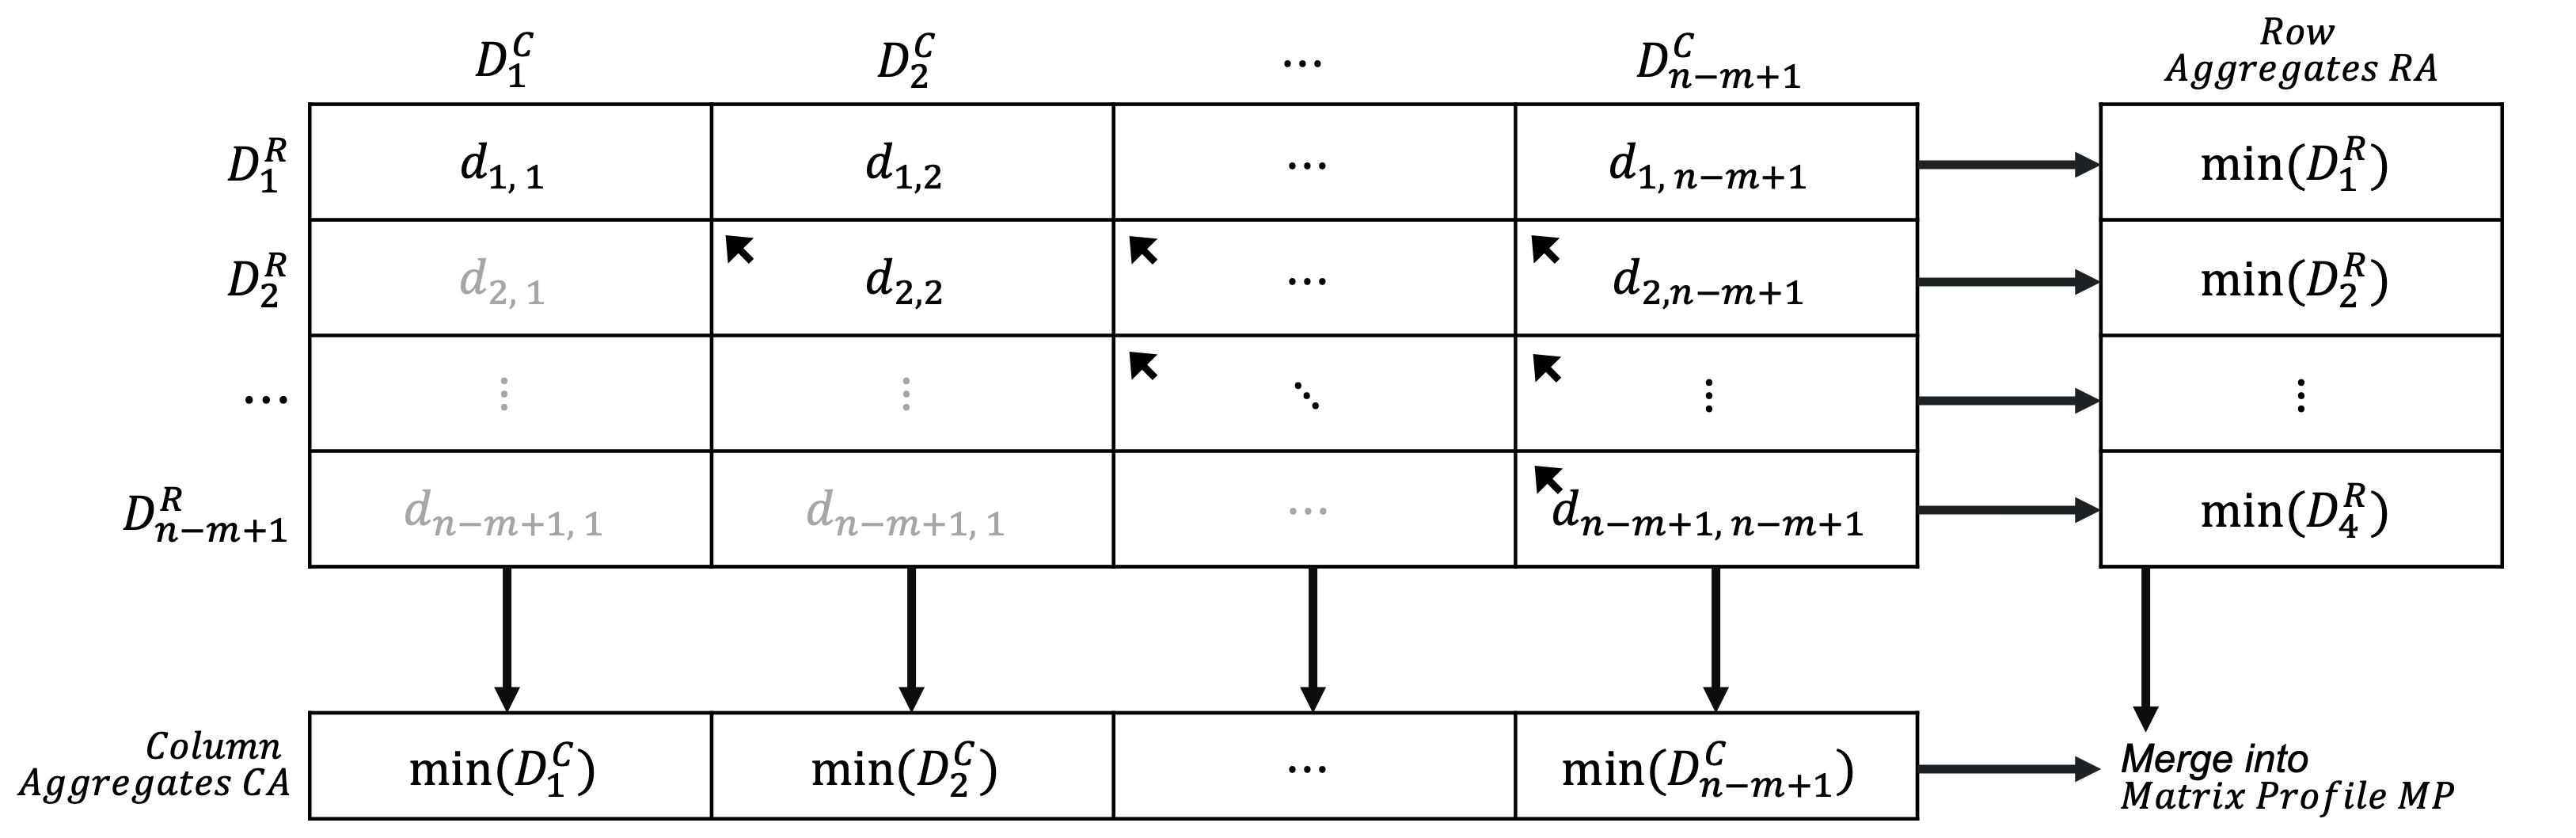
\includegraphics[scale=0.125]{2_2}
    \centering
    \caption{Matrix Profile $MP$ of a Time series $T$ as the column-wise minima of the Distance Matrix and the Matrix Profile Index $MPI$ as the vector of the corresponding indices. In this example, $d_{2,j}$ represents a column-wise minimum and is therefore integrated into the Matrix Profile.}
\end{figure}

The Pearson correlation $P_{i,j}$ between two subsequences $T_{i,m}$ and $T_{j,m}$ of a fixed time series \( T = t_1, t_2, \dots, t_n \) and a common subsequence length \( m \in \mathbb{N} \), as explicitly formulated in Equation 2.2, can be computed as follows:

\begin{equation}
    P_{i,j} = \overline{QT}_{i,j} * inv_i * inv_j
\end{equation}

where,

\begin{equation}
    \overline{QT}_{i,j} = \sum_{k=0}^{m-1}{\left(t_{i+k} - \mu_i\right)\left(t_{j+k} - \mu_j\right)}
\end{equation}

and $inv_k$ denotes the inverse L2-Norm:

\begin{equation}
    inv_k = \frac{1}{||T_{k,m} - \mu_k||}
\end{equation}

SCAMP employes an optimization on $\overline{QT_{i,j}}$ by not implicitly calculation for all $i,j$ by using a centered-sum-of-products formula:

\begin{equation}
    \overline{QT}_{i,j} = \overline{QT}_{i-1,j-1} + df_i \cdot dg_j + df_j \cdot dg_i
\end{equation}

where,

\begin{equation}
    df_k =
    \begin{cases}
        0,                             & \text{if}\ k = 1                 \\
        \frac{t_{k+m-1} - t_{k-1}}{2}, & \text{if}\ 2 \le k \le n - m + 1
    \end{cases}
\end{equation}

and, with $\mu_i$ representing the sample mean of the subsequence $T_{i,m}$,


\begin{equation}
    dg_k =
    \begin{cases}
        0,                                              & \text{if}\ k = 1                 \\
        {t_{k+m-1} + \left(t_{k-1} - \mu_{k-1}\right)}, & \text{if}\ 2 \le k \le n - m + 1
    \end{cases}
\end{equation}

Equations 2.7 and 2.8 are used to precompute the terms used in Equation 2.6 and incorporate incremental mean centering into the update. In addition to $df$ and $dg$, the required L2-norm inverses are precomputed to avoid unnecessary recomputations.\\

As described in Equation 2.1, we can then convert the calculated Pearson correlation into Euclidean distance in $O\left(1\right)$ via:

\begin{equation}
    d_{i,j} = \sqrt{2m\left(1 - P_{i,j}\right)}
\end{equation}


Note, while the computation described in Equation 2.6 introduces a diagonal dependency between computations ($\overline{QT}_{i-1,j-1} \text{ is required to compute } \overline{QT}_{i,j}$), this dependency is circumvented at any point by explicitly calculating $\overline{QT}_{i-1,j-1}$ via the explicit dot product fomulation (Equation 2.4). The explicit caluclation is required for the first row, i.e., $\overline{QT}_{1,j}$ has to be calculated via the straightforward definition.\\
\\
\\
\\
\\
\\
\\
\\
\\
\\


\begin{figure}[h!]
    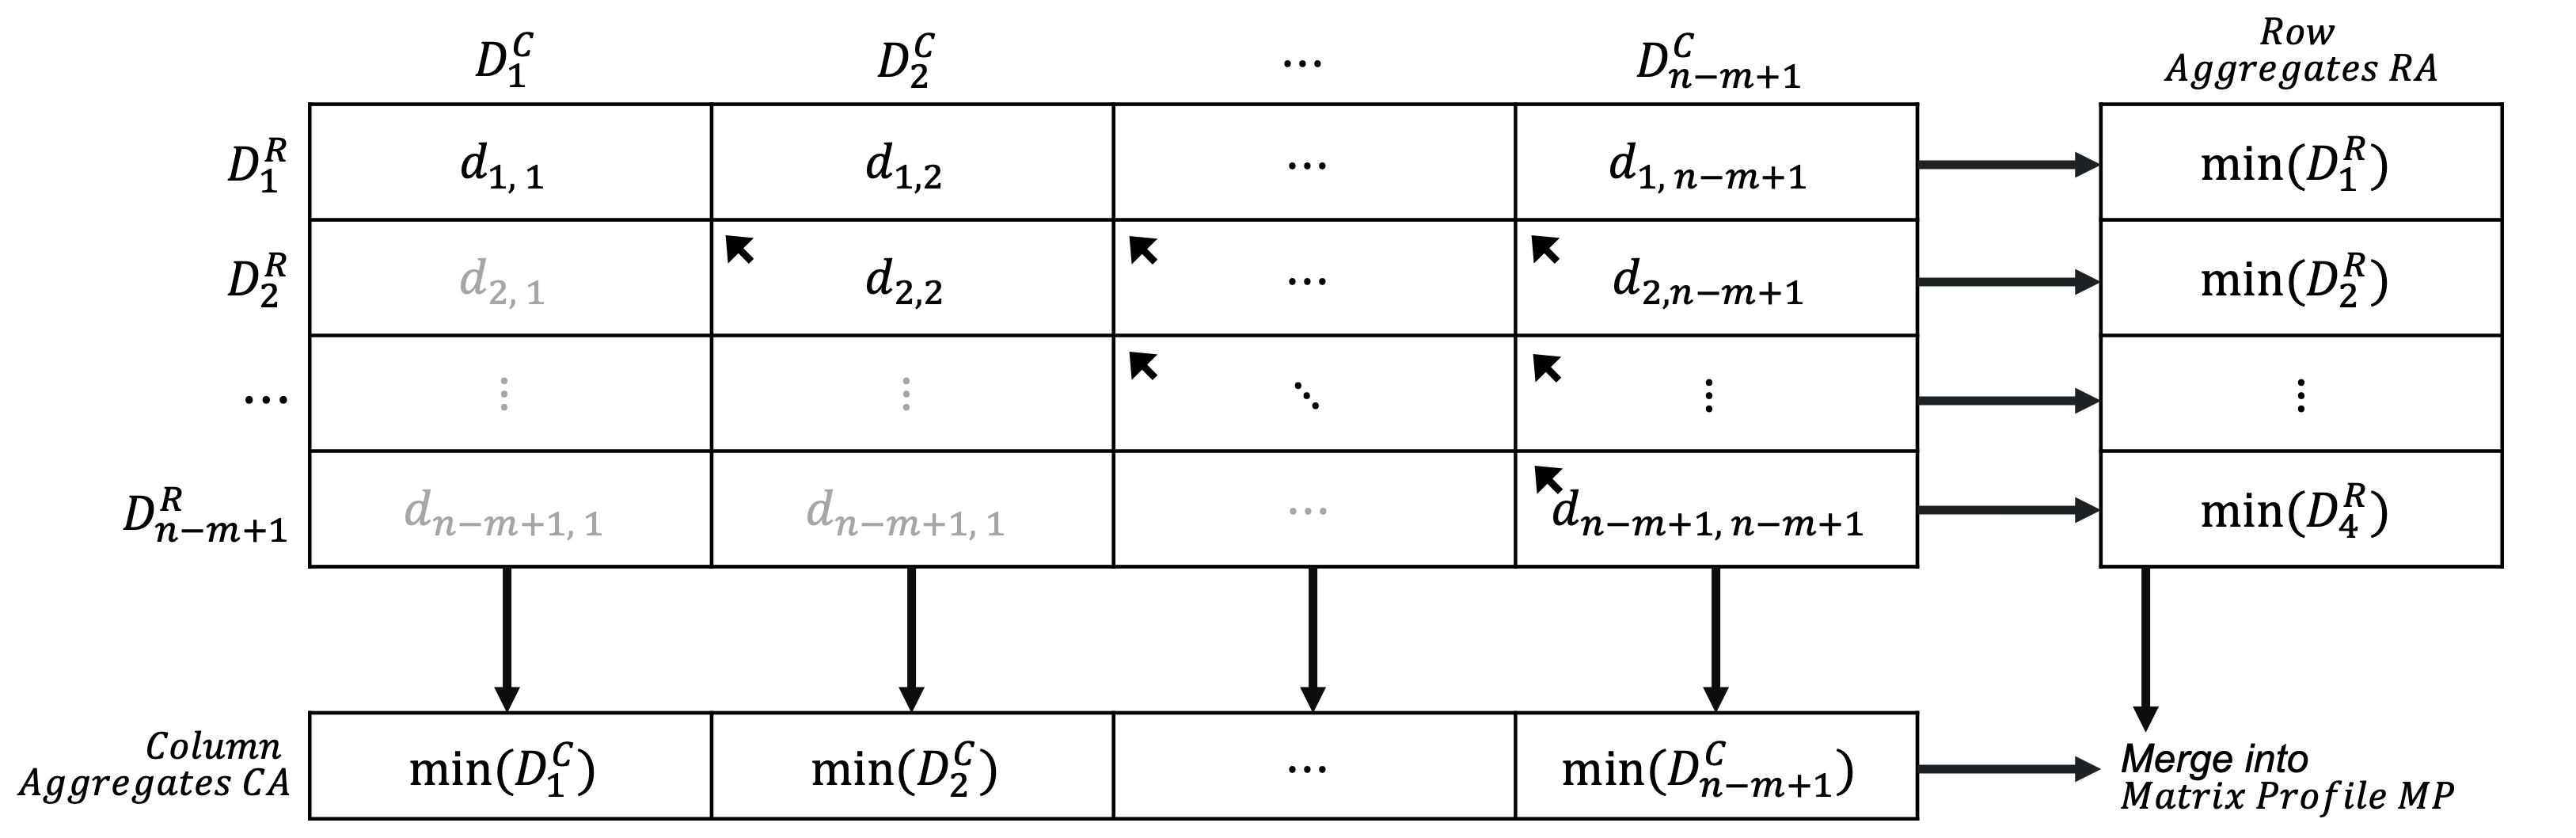
\includegraphics[scale=0.125]{2_3}
    \centering
    \caption{Computation performed by the SCAMP algorithm. In particular, only values
        above (and including) the main diagonal are computed. The diagonal
        dependency introduced through the updated formulation is visualized
        through upward-pointing arrows.}
\end{figure}

SCAMP does not compute the entire matrix but rather only elements above the main
diagonal. This can be done due to the symmetric nature of the problem. We, therefore,
store row- and column-wise aggregates, i.e., the minima of the considered values. These
aggregates are merged subsequently to obtain the resulting matrix profile, as depicted
in Figure 2.3.

\section{Cerebras Wafer Scale Engine}

Cerebras Systems' CS-2 stands as a groundbreaking hardware solution tailored for accelerating deep learning tasks. At its core lies the Cerebras second-generation Wafer Scale Engine (WSE-2), a monumental achievement boasting around 1.2 trillion transistors, making it the largest chip in the industry. The CS-2 wafer operates as a multiple instruction, multiple data (MIMD) distributed-memory system, interconnected via a 2D-mesh fabric. Each fundamental unit on the wafer, referred to as a tile, encompasses a processor core, its memory, and a router facilitating connections. These routers link with neighboring tiles, forming a $7 \times 12$ array housing 84 identical dies, each containing thousands of tiles. Notably, the system integrates 40 gigabytes of on-chip SRAM, offering rapid access within a single clock cycle, alongside staggering memory and interconnect bandwidths of 20 petabytes/sec and 220 petabits/sec, respectively. Comparatively, the WSE-2 dwarfs graphical processing accelerators with over 100 times the compute cores, 1000 times more high-speed on-chip memory, and over 12,000 times more fabric bandwidth. Spanning approximately 46,000 mm$^2$ in size, the WSE-2 employs Sparse Linear Algebra Compute (SLAC) cores for efficient computation, boasting over 850,000 of these cores designed specifically for sparse linear algebra tasks crucial in machine learning. This massive design flexibility empowers the WSE-2 to adapt to various linear algebra paradigms, effectively catering to industry-grade applications. Leveraging SLAC cores enables the WSE-2 to bypass zero-to-zero multiplications in large datasets, optimizing compute resources and system efficiency. The Cerebras Software platform complements this hardware prowess by facilitating seamless machine learning model training, supporting popular frameworks such as TensorFlow and PyTorch. Its graph compiler translates ML models into optimized executables for the CS-2, ensuring smooth integration into researchers' workflows.

\begin{figure}[h!]
    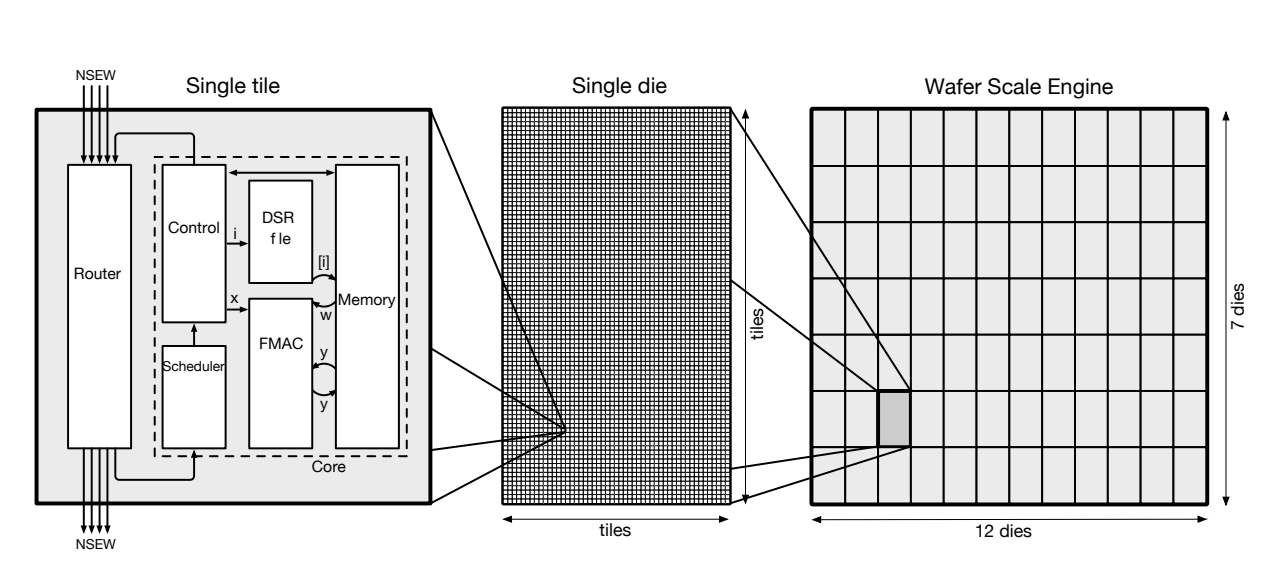
\includegraphics[scale=0.25]{cerebras_wse-2}
    \centering
    \caption{An overview of the Wafer Scale Engine (WSE). The WSE (to the right) occupies an entire wafer, and is a
    2D array of dies. Each die is itself a grid of tiles (in the middle), which contains a router, a processing element and
    single-cycle access memory (to the left). In total, the WSE-2 embeds 2.6 trillion transistors in a silicon area of 46,225
    mm2. \cite{9}}
\end{figure}

The absence of off-chip memory is a distinctive trait of the WSE-2. Unlike other architectures, the WSE-2 doesn't rely on dynamic random access memory (DRAM). Instead, it exclusively employs single-cycle latency static random access memory (SRAM), providing approximately 40 GB of memory. This unique characteristic positions the architecture as a potentially excellent option for HPC simulation kernels that are limited by memory bandwidth or latency. The theoretical bandwidth of the WSE-2 is remarkable, reaching 20 petabytes/second, surpassing the A100 GPU, which typically offers 1.5–2.0 terabytes/second bandwidth depending on the specific model.

The Cerebras System (CS) is a self-contained rack-mounted system containing packaging, power supply, cooling and I/O for a single WSE. The CS communicates via parallel 100 Gigabit ethernet connections to a host CPU cluster. Throughout this documentation, the CS is referred to as the “device,” the host CPU cluster as the “host,” and the ethernet connections connecting the two as “host I/O”. The SDK provides mechanisms for using host I/O to move data between host and device or launch functions on the device.

The below figure gives a visual representation of the mesh of PEs that make up the WSE, and its connections to the outside world. Data is streamed onto the device via host I/O, and enters the WSE through a series of links along its edges. The programming model of the SDK abstracts away the details of these links, and allows the programmer to copy data from the host to arbitrary PEs on the device.

\begin{figure}[h!]
    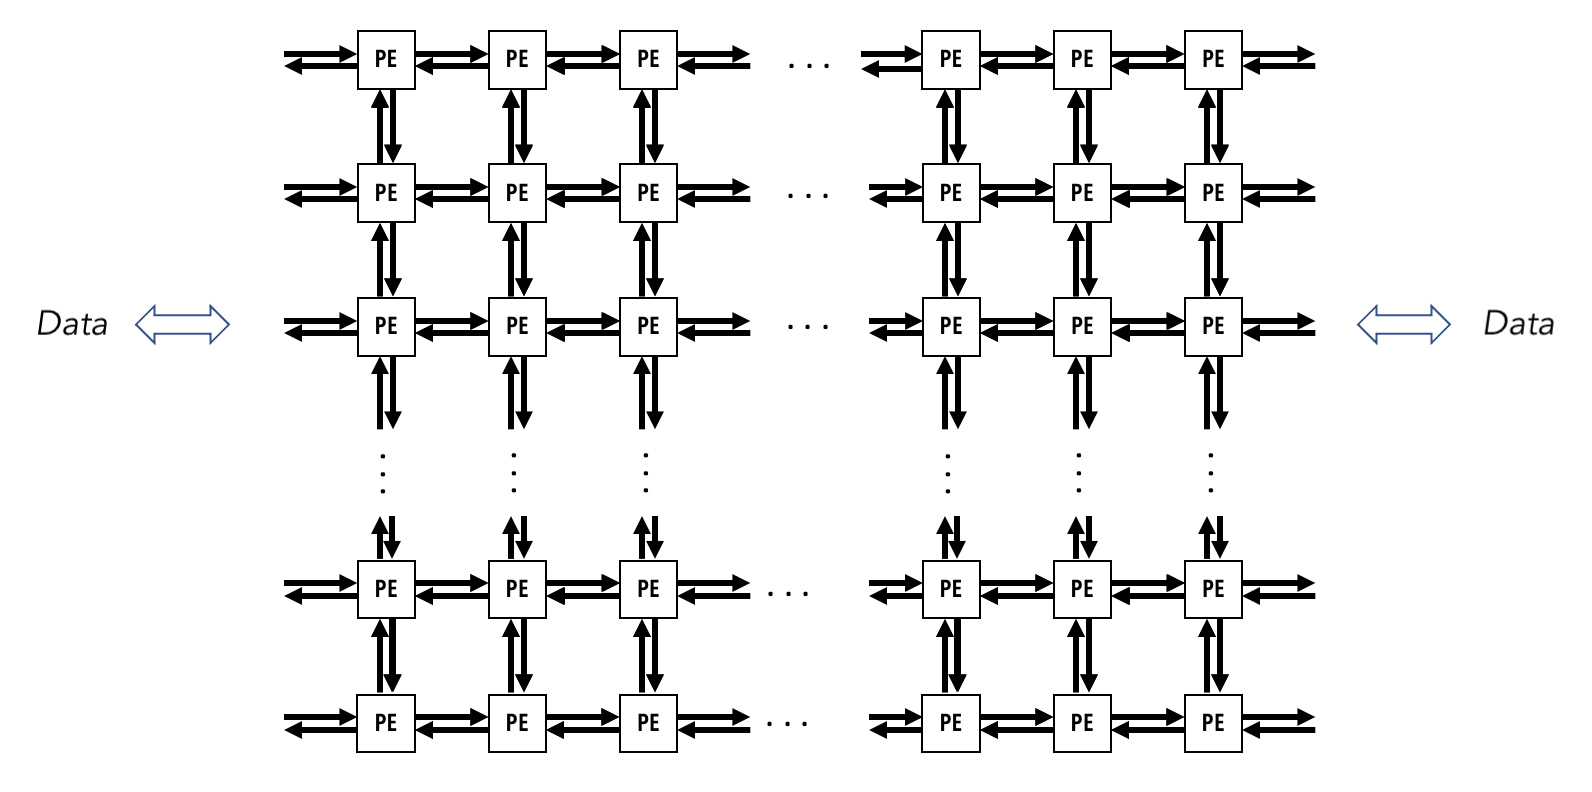
\includegraphics[scale=0.125]{PEs.png}
    \centering
    \caption{The PEs are interconnected cardinally allowing for communication between PEs in packets of size 32 bits.}
\end{figure}


The device allows programmers to interact with the cores using a lower-level code that targets the WSE's microarchitecture directly
using a domain-specific programming language called the Cerebras Software Language, or CSL. In CSL, the cores on the WSE-2 are referred to as Processing Elements (PEs). The programmer
can write code that targets every PE of the wafer such that compute and memory are optimally
utilized. The programmer communicates to the device via a set of runtime APIs executed on one
or more host computers.
Although this device is primarily motivated towards AI workloads, This thesis explores the viability of applying the available hardware and compute power to other diverse workloads like Matrix Profiling.\\

\subsection{Processing Elements}

The 850,000 PEs on the WSE-2 are structured in a 2D grid. Each PE contains a general-purpose compute element (CE), a fabric router, and 48kB of local SRAM memory with single-cycle read/
write access latency. PE-to-PE communication latency is also one cycle. The PE contains a network
router with links to the CE and to the routers of the four nearest PEs in the north, south, east,
and west directions. Communication is integrated into the instruction set, at single 32-bit word
granularity, and is accordingly as fast as arithmetic.
Using the Cerebras SDK, each WSE-2 exposes up to 750×994 user programmable
PEs (i.e., 745,500 PEs). While the WSE-2 hardware actually contains about 850,000
PEs in total, some additional rows and columns around the user-space PEs are reserved for memory movement operations (to facilitate abstractions for moving data
to/from the host) and other system functions
The CE's instruction set supports FP32, FP16, and INT16 data types. The Cerebras ISA supports
optimized vector operations for processing tensors as well as general-purpose control instructions.
A CE can execute vector instructions that perform up to eight operations per clock for FP16
operands.
Each PE is additionaly clocked at 850MHz. Each program is allowed to allocate a certain number of PEs for executing the workload, henceforth, we will refer to this as the \texttt{Resource Rectangle}.

\begin{figure}[h!]
    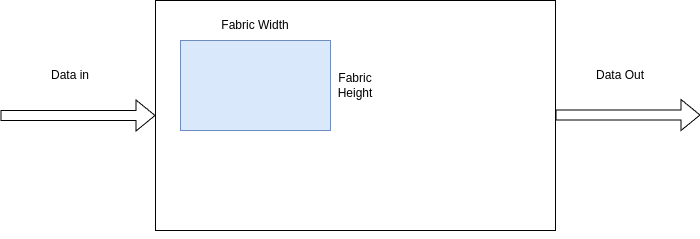
\includegraphics[scale=0.5]{fabric}
    \centering
    \caption{A \texttt{Resource Rectangle}, allocating a partial rectangle of the Wafer for computation}
\end{figure}

\section{Related Works}

The Cerebras WSE-2 has been used by various organisations, including large global corporations, for accelerating machine learning and other purposes. Some interesting AI breakthroughs, the porting of the GPT model to Cerebras \cite{3}, The benefits of accelerating machine learning workloads has been well proven, however there are far fewer studies concerned with using the WSE to run more traditional computational tasks. Already, there have been numerous notable successes from running Stencil computations for solving the 3D wave equation using finite-difference method in seismic imaging applications \cite{5}, fast Fourier transforms for one, two, and three-dimensional arrays \cite{6}, Efficient algorithm for Monte Carlo particle transport \cite{7}, Stencil computations reaching up to 503 TFLOPs on WSE-2, a figure that only full clusters can eventually yield \cite{8}

This work is heavily based on the SCAMP paper introduce by Z. Zimmerman et a \cite{4}. The approach to parallelism introduced and optimized by the SCAMP algorithm could be easy mapped onto the distributed MIMD architecture of Cerebras (See Section 3). When calculating the Matrix Profile aggregates of a row or column, the algorithm does not contain any data dependency across rows or columns which allows us to exploit weak scaling which the Cerebras system is aimed at. This form of algorithm is widespread in scientific computing and hence represents the underlying computational pattern in use by a large number of HPC codes.
